%%****************************************************************************
%** Copyright 2002, 2003 by Lukas Ruf, <ruf@topsy.net>
%** Information is provided under the terms of the
%** GNU Free Documentation License <http://www.gnu.org/copyleft/fdl.html>
%** Fairness: Cite the source of information, visit <http://www.topsy.net>
%****************************************************************************
%** Last Modification: 2005-07-11 1600
%** 2005-07-11	Bernhard Tellenbach
%**							Switched default document class to: book
%**							Added %%****************************************************************************
%** Copyright 2005 by Bernhard Tellenbach, <bernhard.tellenbach@airmail.ch>
%** Information is provided under the terms of the
%** GNU Free Documentation License <http://www.gnu.org/copyleft/fdl.html>
%****************************************************************************
%****************************************************************************
%** Last Modification: 2005-07-11 1600
%** 2005-07-11	Updated the syntax to match the current nomencl packet
%****************************************************************************

\chapter{\label{appendixA}Title}


\section{\label{chapterA:section1}Section 1}

\begin{verbatim}
All is presented exactely the way you write it.

Page boundaries are not checked.....................................................................................

\end{verbatim}

\chapter{\label{appendixB}Title}


%Entries for the list of abbrevations:
%
%To generate the list of abbrevations, execute:
%makeindex Thesis.nlo -s nomencl.ist -o Thesis.nls
%
%If you are using TeXniCenter, specify:
%"%bm.nlo" -s nomencl.ist -o "%bm.nls"
%as beeing the argument list for makeindex.
%---------------------------------------------------------------------------------------------------------
%For old nomencl package uncomment this:
%\printglossary
%For new nomencl package uncomment this:
\printnomenclature

\abbrev{XCA}{\markup{X}tremely \markup{C}ool \markup{A}bbrevations}



%****************************************************************************

\documentclass[12pt,final,a4paper,twoside]{book}
%\documentclass[12pt,draft,a4paper,twoside]{book}
%\documentclass[10pt,draft,a4paper,oneside]{report}
%\documentclass[10pt,draft,a4paper,oneside]{article}

%**Latex Master Document*********

%** preamble.tex: here all the document-wide settings
%                 are defined
%****************************************************************************
%** Copyright 2001, 2002, 2003, 2004 by Lukas Ruf, <lukas.ruf@lpr.ch>
%** Information is provided under the terms of the
%** GNU Free Documentation License <http://www.gnu.org/copyleft/fdl.html>
%** Fairness: Cite the source of information, visit <http://www.topsy.net>
%****************************************************************************
%** Last Modification: 2005-07-11 1600
%** 2004-02-17: Lukas Ruf
%**             Added recommendation by Thomas Duebendorfer
%**             Added different babel languages
%**             Added more comments
%** 2004-10-16: Lukas Ruf
%**             More comments
%**             Added subfigure
%** 2005-07-11	Bernhard Tellenbach
%**							Added \abbrev command to generate a list of abbrevations
%**							Removed support for psfig and epsfig (old)
%** 						Adapted syntax for new nomencl packet version
%****************************************************************************

\RequirePackage{times}

\usepackage[english]{babel}
%-% \usepackage[german]{babel}
%-% \usepackage[ngerman]{babel}

\usepackage[latin1]{inputenc}
\usepackage[T1]{fontenc}
\usepackage{type1cm}

\usepackage{a4}

\usepackage[dvips]{graphicx}
\graphicspath{{Figures/},{Pictures/}}
\usepackage{subfigure}

\usepackage{fancyhdr}
\usepackage{fancybox}

\usepackage{float}
\usepackage{longtable}
\usepackage{paralist}
\usepackage{url}
\usepackage{portland}
\usepackage{lscape}
\usepackage{moreverb}

\usepackage{nomencl}
  \let\abbrev\nomenclature
  \renewcommand{\nomname}{List of Abbrevations}
  \setlength{\nomlabelwidth}{.25\hsize}
  \renewcommand{\nomlabel}[1]{#1 \dotfill}
  \setlength{\nomitemsep}{-\parsep}
  %For old nomencl package, uncomment this:
  \makeglossary 
  %For new nomencl package, uncomment this:
  %\makenomenclature

\usepackage[normalem]{ulem}
  \newcommand{\markup}[1]{\uline{#1}}
  
   
%% Thanks to Thomas Duebendorfer: Should create smoother fonts
\usepackage{ae,aecompl}


\usepackage[first,bottomafter,light,dvips]{draftcopy}
\draftcopyName{Draft v0.1}{120}

\addtolength{\textwidth}{2cm}
\addtolength{\textheight}{2cm}
\addtolength{\oddsidemargin}{-1.0cm}
\addtolength{\evensidemargin}{-1.0cm}
\addtolength{\topmargin}{-1.5cm}

%% No Serifs: Put comment markers in front of the next three lines otherwise
\renewcommand{\ttdefault}{cmtt}
\renewcommand{\rmdefault}{phv}  % Helvetica for roman type as well as sf
\renewcommand{\ttdefault}{pcr}  % use Courier for fixed pitch, if needed

\newcommand{\?}{\discretionary{/}{}{/}}
\newcommand{\liter}[0]{/home/ruf/Lib/Bibl/}
\newcommand{\fref}[1]{\mbox{Figur~\ref{#1}}}

\pagestyle{fancy}
%%-lpr Note: 'chapters' are defined for 'book's only
%%-lpr       in articles, we make use of sections only
%%-lpr \renewcommand{\chaptermark}[1]{\markboth{#1}{}}
\renewcommand{\sectionmark}[1]{\markright{\thesection\ #1}}
\fancyhf{}
\fancyhead[LE,RO]{\bfseries\thepage}
\fancyhead[LO]{\bfseries\rightmark}
\fancyhead[RE]{\bfseries\leftmark}
\renewcommand{\headrulewidth}{0.5pt}
\addtolength{\headheight}{0.5pt}
\fancypagestyle{plain}{%
   \fancyhf{}
   \fancyfoot[C]{\bfseries \thepage}
   \fancyhead{}%get rid of headers on plain pages
   \renewcommand{\headrulewidth}{0pt} % an the line
}
\newcommand{\clearemptydoublepage}{\newpage{\pagestyle{empty}\cleardoublepage}}

\setlength{\parindent}{0in}

\hyphenation{Lukas not-to-hyphen-else-where}

\newcommand{\Appendix}[2][?]
{
  \refstepcounter{section}
  \addcontentsline{toc}{appendix}
  {
    \protect\numberline{\appendixname~\thesection} %1
  }
  {
    \flushright\large\bfseries\appendixname\ \thesection\par
    \nohypens\centering#1\par
  }
  \vspace{\baselineskip}
}

\let\margin\marginpar
\newcommand\myMargin[1]{\margin{\raggedright\scriptsize #1}}
\renewcommand{\marginpar}[1]{\myMargin{#1}}

\newcommand\CHECK{\myMargin{CHECK}}
\newcommand\NEW{\myMargin{NEW}}

%********************************

%** begin the document environment
\begin{document}


\frenchspacing
\sloppy

%** Title.tex: Title page to be printed first
  %****************************************************************************
  %** Copyright 2002 by Lukas Ruf, ruf@topsy.net
  %** Information is provided under the terms of the
  %** GNU Free Documentation License http://www.gnu.org/copyleft/fdl.html
  %** Fairness: Cite the source of information, visit http://www.topsy.net
  %****************************************************************************
  %** Extensions:
  %** January 2003: Thomas Duebendorfer <thomas@duebendorfer.ch>
  %**   changed the former ETH Header to the new, official one that is
  %**   mandatory since January 2003.
  %****************************************************************************
  %****************************************************************************
  %** Extensions:
  %** January 2005: Bernhard Tellenbach <bernhard.tellenbach@airmail.ch>
  %**   changed the way the ETH Header is included. Slight modification of the
  %**   content.
  %****************************************************************************
  \begin{titlepage}

  \begin{center}
  \begin{figure}[!t]
     
\includegraphics{TIKETHhdr.eps}
  \end{figure}
  \end{center}

  \vspace{2 cm}

  {\large FirstName Name}
  \vspace{2 cm}

  {\Huge Thesis Title}\\

  \vspace{\fill}


  (Master/Semester) Thesis (MA/SA)-20XX-XX\\
  July 2005 to January 2006\\

  \vspace{1cm}
  Tutor: \\
  Co-Tutor: \\
  Supervisor: \\
    
  \end{titlepage}


%** environments.tex: Predefined Environments
%****************************************************************************
%** Copyright 2002 by Lukas Ruf, ruf@topsy.net
%** Information is provided under the terms of the
%** GNU Free Documentation License http://www.gnu.org/copyleft/fdl.html
%** Fairness: Cite the source of information, visit http://www.topsy.net
%****************************************************************************

\newenvironment{sourcecode}%
{\vspace{0.5 cm} \footnotesize \verbatim}%
{\endverbatim \normalsize \vspace{0.5 cm}}

\newenvironment{inputverb}[1]%
{\vspace{0.5 cm} \footnotesize \verbatiminput{#1}}%
{\normalsize \vspace{0.5 cm}}

\newenvironment{inputverb_nospace}[1]%
{\footnotesize \verbatiminput{#1}}%
{\normalsize}



%**Documentation****************

%** Abstract.tex: Contains a brief description
%                 of what the reader may expect
%%****************************************************************************
%** Copyright 2002 by Lukas Ruf, ruf@topsy.net
%** Information is provided under the terms of the
%** GNU Free Documentation License http://www.gnu.org/copyleft/fdl.html
%** Fairness: Cite the source of information, visit http://www.topsy.net
%****************************************************************************
%** Last Modification: 2005-07-11 1600
%** 2005-07-11	Bernhard Tellenbach
%**							Inserted new content
%****************************************************************************
\clearpage
\null
\vfil % or it might be \null
\begin{center}\textbf{Abstract}\end{center}
In journal articles, research papers, published patent applications and patents, an abstract is a short summary placed prior to the introduction, often with different line justification (blockquote) from the rest of the article, used to help readers determine the purpose of the paper. While the length of the abstract varies by field of study, it is typically a paragraph in length (3-5 sentences), and never more than a page. See
\emph{en.wikipedia.org/wiki/Abstract\_(summary)} for details
\vfil
\clearpage 



%** Table of Contents
\tableofcontents

%** Table of Figures
%\listoffigures

%** Table of Figures
%\listoftables

%** Introduction.tex: Contains an introduction to
%                     the topic and motivates the work.
%                     State what the reader can find where.

\chapter{\label{introduction}Introduction}

\section{Motivation}

The increasing number and diversity of networking devices is challenging the network research community. More and more applications and protocols are developed to address the needs of different platforms and use cases. For performance reasons, these protocols and applications are often tightly bound to each other. The resulting systems may then perform well, but lack of flexibility in the underlying architecture. This inflexibility is well demonstrated by the long lasting and still ongoing switch from IPv4 to IPv6 in the TCP/IP protocol stack of the current Internet architecture.

The Autonomic Network Architecture~(ANA)~\cite{ana} targets this problem with a fundamental change of paradigms. In ANA, all functionality is encapsulated in so called functional blocks. The size of functional blocks is a priori not defined. It may range from a minimalistic checksum calculation up to a huge holistic protocol stack. ANA provides a set of abstraction models and generic communication methods that the functional blocks use to interact with each other. This framework allows a completely isolated development of the algorithms running in the functional blocks. The operating system then interconnects the functional blocks and builds up an individual protocol stack. The device chooses the functional blocks for this protocol stack depending on the capabilities of the platform and the requirements of the running applications. The result is a flexible and dynamic protocol stack, that is able to adapt itself to any given situation and may change at runtime. Figure~\ref{protocolStack.eps} shows such a dynamic protocol stack and compares it to the inflexible, static and strongly layered protocol stack of the current Internet.

\begin{figure}
  \begin{center}
		 \includegraphics[scale=1.3]{protocolStack.eps}
  \caption{a) The strongly layered static protocol stack of the current Internet, b) The dynamically adaptable protocol stack of an ANA node}
  \label{protocolStack.eps}
  \end{center}
\end{figure}
The existing implementations of ANA \cite{ana}, \cite{lana} do not yet reach the performance of the traditional Internet architecture. This is due to two reasons. First of all, the level of indirection introduced by ANA trades some performance optimization features of the application for a higher flexibility and modularity of the overall system. The second reason is that the traditional Internet architecture benefits from a wide range of hardware support in the networking interface cards, which is not yet available for ANA. In order to compensate the performance penalty of ANA, a hardware acceleration for ANA is needed. It is not feasible to use application specific integrated circuits~(ASIC) for this purpose, since the functionality of these devices must be completely specified at design time. This static characteristic of ASICs would conflict with ANA's effort towards flexibility and adaptability.

The evolving partial reconfiguration capabilities of modern field programmable gate arrays (FPGA) combine the flexibility of a software implementation with the high-performance acceleration features of ASICs. L\"{u}bbers et. al.~\cite{towardsAdaptiveNetworkingForEmbeddedDevices} and Keller et. al.~\cite{reconfigurableNodesForFutureNetworks} therefore came up with the idea of porting ANA to a reconfigurable system on chip (rSoC). On these devices, a microprocessor core (either soft- or hardcore)  is combined with a programmable logic fabric. The software running in the microprocessor may then decide to offload the execution of computational intensive and frequently used functional blocks from the microprocessor to the programmable logic. Based on the partial reconfiguration features, this mapping of functional blocks to hardware or software can be adapted at runtime.

In order to reduce the engineering effort, L\"{u}bbers et. al.~\cite{towardsAdaptiveNetworkingForEmbeddedDevices} and Keller et. al.~\cite{reconfigurableNodesForFutureNetworks} further suggest to use ReconOS~\cite{reconos} as base system. In ReconOS, partially reconfigurable logic slots are used as so called hardware threads. These hardware threads appear to the software like normal software POSIX-threads. ReconOS enables the hardware threads to access operating system objects like semaphores, message boxes and shared memory. The combination of these mechanisms simplifiess the interaction of software and hardware elements. The suggested approach benefits from the hardware acceleration provided by ReconOS by implementing some functional blocks as hardware threads. Figure~\ref{reconosForAna.eps} shows the architecture of ReconOS and how the functional blocks are mapped to the hardware threads.

\begin{figure}
  \begin{center}
		 \includegraphics[width=\textwidth]{reconosForANA.eps}
  \caption{a) The ReconOS architecture: partially reconfigurable logic slots are used as hardware threads. b) Using ReconOS for ANA: a set of functional blocks is executed in hardware threads.}
  \label{reconosForAna.eps}
  \end{center}
\end{figure}
However, the major problem of this approach is the shared bus architecture of ReconOS. Especially with a data intensive application like ANA, the shared bus soon becomes the bottleneck of the system. 

\section{Aims of this Thesis}
In this thesis we present an extension of the ReconOS framework with a high-throughput communication infrastructure shown in figure~\ref{interconnectionInfrastructure.eps}. This infrastructure contains a packet based network on chip (NoC) that guarantees each hardware thread a worst-case incoming and outgoing data throughput. Additionally, a ring buffer based gateway is designed and implemented to speed up the transfer from software to hardware and vice versa.

\begin{figure}
  \begin{center}
		 \includegraphics[width=\textwidth]{interconnectionInfrastructure.eps}
  \caption{The high throughput communication interface guarantees the functional blocks a worst case incoming and outgoing bandwith.}
  \label{interconnectionInfrastructure.eps}
  \end{center}
\end{figure}

\section{Organization of the Thesis}
The reminder of this thesis is organized in the following way: TODO!

%** Problem.tex: Documentation in own words of the problem to
%                be addressed in this document:
%                What is the challenge, why is it useful what you
%                plan to do.
%%****************************************************************************
%** Copyright 2002 by Lukas Ruf, ruf@topsy.net
%** Information is provided under the terms of the
%** GNU Free Documentation License http://www.gnu.org/copyleft/fdl.html
%** Fairness: Cite the source of information, visit http://www.topsy.net
%****************************************************************************
%****************************************************************************
%** Last Modification: 2005-07-11 1600
%** 2005-07-11	Bernhard Tellenbach
%**							This is an addapted version of the Introduction.tex file
%**							Added table example (footnotes,multicolumn)
%**							Examples for different text sizes
%**							Updated eps file inclusion example for use with graphicx pkt. 
%****************************************************************************

\chapter{\label{chapter2}Title}
In \ref{introduction} we start with our introduction to the problem that we 
are going to address.  Since we do not want to waste the readers time we 
go and show the essential issues of latex in section
\ref{chapter2:essentials}.

\section{\label{chapter2:essentials}Essentials}

Well this section can be further subdivided into subsection.  We present 
this in subsection \ref{chapter2:essentials:subsections}.

\subsection{\label{chapter2:essentials:subsections}Subsections}

\paragraph{\label{introduction:essentials:subsections:paragraph}Paragraphs}
can be specially referenced as well.

Of further importance is the understanding of the following environments:

%*** itemized lists
\begin{itemize}
\item This shows an itemized bullet list
  \begin{itemize}
  \item Which can be used for several levels\ldots
  \end{itemize}
\end{itemize}

%*** enumerated lists
\begin{enumerate}
\item The same applies to enumerated lists.
\end{enumerate}

\begin{figure}[!hbt]
  \begin{center}
		 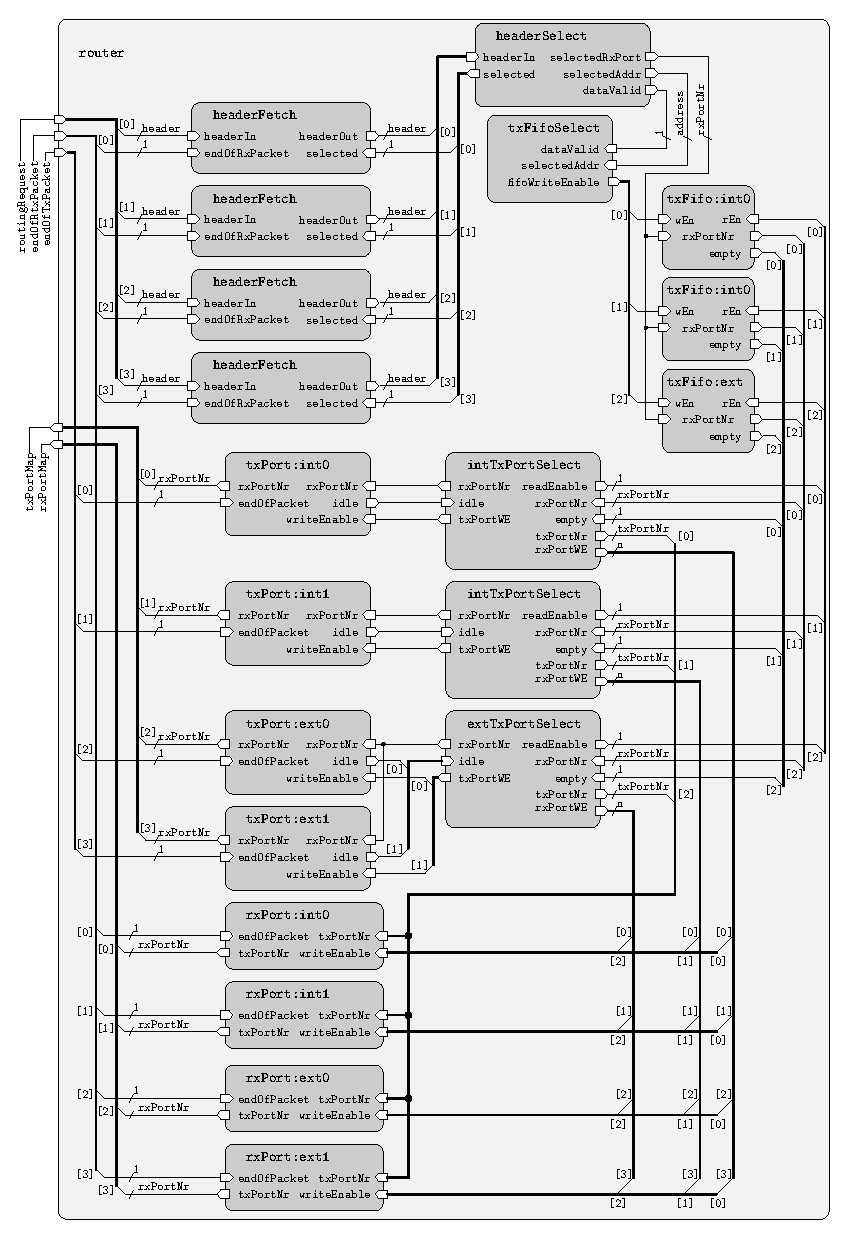
\includegraphics[width=\textwidth]{router.eps}
  \caption{This is a figure to be printed in a float}
  \label{router.eps}
  \end{center}
\end{figure}
By figure \ref{router.eps}, we show some funny figures.


Table with caption and footnotes below the table.

\begin{table}[htbp]
\begin{center}\begin{minipage}{\textwidth}
\begin{tabular}{| c | p{130pt} | l |}
\hline
Column 1 & Column 2 \newline (additional line) & Column 3 \\
\hline
C1,R2 & C2,R2 & C2,R3 \\
\hline
C1,R3	& \multicolumn{2}{| c |}{C2\&C3,R3} \\
\hline
C1,R4 & C2,R4\footnote{Footnote to table~\ref{tab:table1}} & C3,R4\\
\hline
\end{tabular}
\end{minipage}
\caption{Table 1}
\label{tab:table1}
\end{center}
\end{table}

Examples of different text sizes:

\small Small \\
\scriptsize Script size \\
\normalsize Normal \\
\large Large \\
\huge Huge \\
\normalsize

\CHECK
If we reference to another document, we cite the document \cite{bib:relevantwork}.

%** landscape
\NEW
\begin{landscape}
Of some interest is also the landscape environment:
\end{landscape}

\verbatiminput{filename.txt}
Even though we don't think full listings are useful in documents,
you can easily insert complete files by the verbatiminput{}-command.



%** Design.tex: How was the problem attacked, what was the design
%               the architecture 
\chapter{\label{design}Design}

We start this chapter by introducing the design goals of the ReconOS extension in section \ref{designGoals}. This is followed by an evaluation of architectures and NoC topologies in the sections \ref{evaluationOfDesignPrinciples} and \ref{evaluationOfTopologies}, respectively. Section \ref{hwSwDataTransfer} describes the design of the hardware/software data transfer mechanism.

\section{\label{designGoals}Design Goals}

In ReconOS, multiple hardware threads can execute tasks independent of the CPU. To this end, the hardware threads and software running in the CPU still need to exchange data with each other. ReconOS provides different mechanisms for this purpose, most notably message boxes and shared memory. All of these mechanisms have in common that they use a shared bus for data transmission. This shared bus architecture is not well suited for networking applications like ANA. Imagine a packet that has to be processed by a set of functional blocks, all of them mapped to hardware threads. In this case, the bus has to repeatedly forward the whole packet from one functional block to the next. The overall data transfer on the bus therefore increases linearly to the number of participating functional blocks.

In this thesis, we want to extend the ReconOS architecture with a high-throughput communication infrastructure. The data rate at which each functional block can send data over the communication infrastructure to a specific destination should be independent of the traffic passing by targeting a different destination.

We distinguish three different applications of data transfer:
\begin{itemize}
	\item Data transfer from a hardware thread to a software thread
	\item Data transfer from a software thread to a hardware thread
	\item Data transfer from one hardware thread to another hardware thread
\end{itemize}
The case of data transfer from one software thread to another software thread is out of the scope of this thesis.

ANA processes packets in two distinct directions. \textit{Ingress} packets arrive at the physical interface, traverse the protocol stack upward and finally reach the corresponding application. \textit{Egress} packets have their origin in the application layer, traverse the protocol stack downwards and then leave the device on the physical interface.

\paragraph{Throughput}
In this thesis, we assume that the size of a packet does not significantly change on its way through the protocol stack. We can therefore set an upper bound of the total data rate at the input and output port of each functional block. This upper bound is equal to the data rate of the physical interface. In our development environment we use a Xilinx ML605 evaluation kit~\cite{ml605}. Its physical interface is a Gigabit Ethernet Module.

We therefore specify the following requirement for the communication infrastructure: The outgoing data rate of each functional block is upper bounded by 1 Gigabit/s. The communication infrastructure then forwards 1 Gigabit/s of data to each hardware-mapped functional block, independently of the origin of the data.

\paragraph{Latency}
Data transfers that cross the hardware/software boundary cause an orders of magnitudes higher latency than data transfers in the hardware domain~\cite{reconfigurableNodesForFutureNetworks}. This is caused by shared memory access and by the high overhead of unavoidable interrupts. The total latency of an ingress or egress of packet is therefore mainly influenced by the performance of the hardware to software or software to hardware data transfer, respectively. We therefore neglect latencies caused by the communication infrastructure between hardware threads and focus on the latencies induced by crossing the hardware/software boundary.

\paragraph{Hardware Resource Utilization}
The desired communication infrastructure is only a helper construct for the actual application running on the device. Hence, we want to keep it as small as possible, so that there is a maximum of programmable logic still available for the application.

\section{\label{evaluationOfDesignPrinciples}Evaluation of Architectures}
In this section, we discuss possible design principles for the communication infrastructure. The discussion is based on the results of Lee et. al.~\cite{communicationArchitectureExploration}. In subsection~\ref{designPrinciples:conclusion}, we then conclude which design principle best fits to the design goals stated in section \ref{designGoals}.

\subsection{\label{evaluation:p2p}Point to Point Interconnection (P2P)}
In a P2P architecture, all hardware threads are directly connected to each other. The data transmission rate and the latency is optimal, since the packets do not need to share resources with any other transmission. The receiving hardware thread is responsible for the serialization of packets that concurrently arrive on different input ports. Lee et. al.~\cite{communicationArchitectureExploration} show that the logic and routing resource utilization of this architecture scales very bad with an increasing number of peers.

\subsection{Multibus}
The multibus architecture is a mixture of the original shared bus architecture of ReconOS and the P2P architecture. In this architecture, all hardware threads read from their own individual bus. In order to send a packet to a hardware thread, the source hardware thread writes the packet to the bus of the destination hardware thread. An individual bus arbiter is required for each hardware thread.

The data rate on this architecture is optimal, since each hardware thread can receive data with the full data rate of its bus. The latency depends on the response time of the bus arbiter. Since all hardware threads have their own bus that must connect to each hardware thread, we assume that this architecture has a high routing resource utilization. We further assume, that the long bus wires and the parasitic capacities of the high impedance bus interfaces limit the clock rate on the bus when the number of hardware threads increase.

\subsection{\label{evaluation:noc}Network on Chip (NoC)}
A NoC is a packet based communication architecture. Intellectual property (IP) cores (hardware threads in the context of ReconOS) are connected to a dedicated switch. The switches are then interconnected with each other according to a selected topology. When a packet arrives on an incoming link of a switch, the switch selects an outgoing link depending on the packet's header and forwards the packet on this link.

A NoC is subject to many configuration issues, e.g. the topology, the number of IP cores per switch or the routing policy. This configuration possibility enables the developer to adapt the NoC architecture to any given requirements.

The latency of the packets and the flow through the network strongly depend on the selected topology and the routing policy. The NoC architecture has a higher latency compared to the Multibus architecture. The reason for this is that the packets must traverse the network hop by hop. Thereby every hop induces a latency of one clock cycle and possibly an additional latency caused by the routing mechanism. On the other hand, the length of the hop signals~-~and with this also their clock rate~-~is independent of the number of IP cores. This is not the case for the Multibus architecture. We can therefore state, that the NoC architecture scales better with increasing number of hardware threads than the Multibus architecture.

\subsection{\label{designPrinciples:conclusion}Conclusion}
Based on the discussion in subsections \ref{evaluation:p2p} to \ref{evaluation:noc}, we assigned grades from 1 to 10 to each presented architecture. The total grade of the architectures is a weighted average of the individual grades. The grades are:
\begin{itemize}
	\item \textbf{Data Rate} (weight 5): The average throughput of the architecture. 10 is the highest throughput.
	\item \textbf{Latency} (weight 2): The average latency of the packets. 10 is the lowest latency.
	\item \textbf{Chip Area} (Weight 3): The expected chip area consumed by the architecture. 10 is the smallest chip area.
	\item \textbf{Engineering Effort} (weight 2): The engineering effort for developing an implementation of the architecture. 10 is the least effort (e.g. ReconOS as is).
	\item \textbf{Scalability} (weight 4): The scalability of the architecture in all the above mentioned criteria for an increasing number of hardware threads. 10 is the best scalability.
\end{itemize}
The assigned grades are shown in figure \ref{evaluationOfDesignPrinciples.eps}.
\begin{figure}
  \begin{center}
		 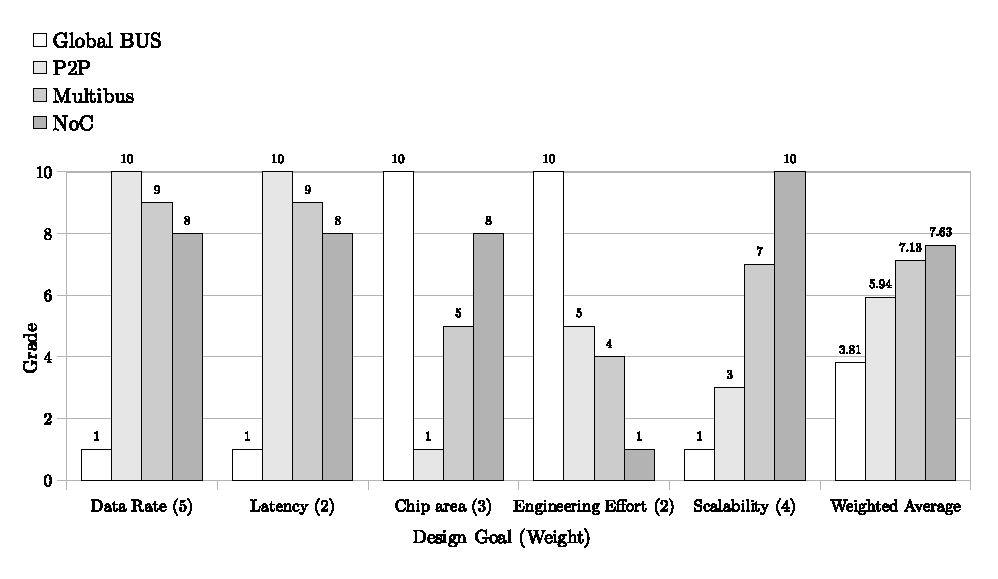
\includegraphics[width=\textwidth]{evaluationOfDesignPrinciples.eps}
  \caption{For each design goal a grade ranging from 1 to 10 is assigned to each architecture. The weighted average of the grades represents the overall suitability of the architectures for the problem at hand.}
  \label{evaluationOfDesignPrinciples.eps}
  \end{center}
\end{figure}
As we expected, the global bus architecture (weighted average 3.81) and the P2P architecture (weighted average 5.94) get significantly lower grades than the Multibus architecture (weighted average 7.13) and the NoC architecture (weighted average 7.63). The higher weighted average of the NoC architecture compared to the Multibus architecture is mainly due to the better scalability.

Based on these results, we decided to implement the communication infrastructure as NoC. An evaluation of NoC topologies is presented in section \ref{evaluationOfTopologies}.





\section{\label{evaluationOfTopologies}Evaluation of NoC Topologies}
The performance of a NoC heavily depends on the topology used to interconnect the switches and the corresponding routing policy. In this section, we first present the evaluated topologies and routing mechanisms in subsection~\ref{evaluationOfTopologies:topologies}. Subsection \ref{linkFlowMeasure} then presents the \textit{total link flow} measure used to estimate the resources consumed by the links of a given NoC topology. In subsection \ref{evaluationOfTopologies:conclusion}, we then conclude which topology fits the requirements best.

In this thesis we ignore load balancing since any benefit from this approach would be cancelled out by the worst-case traffic pattern.

\subsection{\label{evaluationOfTopologies:topologies}Topologies and Routing Policies}
The topology of an NoC describes how the switches are interconnected with each other and how the functional blocks are connected to the switches. The routing policy specifies the outgoing link of a switch on which an incoming packet is forwarded depending on the destination address of the packet. The topology is specified at design time and does not change at runtime. Each switch has therefore a global knowledge on the topology and can use this knowledge for the routing decision.

\paragraph{Grid topology}
In the grid topology, the switches are arranged in a mesh. Figure~\ref{nocTopologies.eps}~a) shows an example of the grid topology. We evaluated this topology with the xy-routing policy. In this routing policy, an x- and an y-coordinate is assigned to each switch. The switches forward packets in the x-dimension until the x-coordinate of the destination address and the x-coordinate of the processing switch is equal. The switches then forward the packets in the y-dimension until the packet reaches its destination.

An advantage of the grid topology is, that it is easily mappable to the available chip area. A big drawback is that it is not applicable to all possible number of functional blocks. If the number of functional blocks is not a square number, the resulting topology will not be optimal.

\paragraph{Torus topology}
The torus topology is build in the same way as the grid topology with the exception that border switches are also interconnected. An example of the torus topology is shown in figure~\ref{nocTopologies.eps}~b). For the torus topology we also used the xy-routing policy. The advantages and disadvantages of the torus topology are much the same as for the grid topology.

\paragraph{Ring topology}
In the ring topology, the switches are arranged in a ring as shown in figure~\ref{nocTopologies.eps}~c) and d). We distinguish two different routing policies: \textit{unidirectional} routing and \textit{bidirectional} routing. Switches using the unidirectional routing policy forward all packets to the same switch. Therefore all packets travel in the same direction, e.g. clockwise. Switches using the bidirectional routing mechanism first determine the number of hops to the destination of the packet in the clockwise and anticlockwise direction. They then send the packet in the direction where the number of hops is smaller.

We further extend the ring topology by connecting multiple functional blocks to the switches. The destination address of the packets then consists of a \textit{global address} and a \textit{local address}. The global address represents the switch to which the destination functional block is connected. The local address identifies the functional block in the set of functional blocks connected to the same switch. The combination of global and local addresses is then unique within the NoC.

The routing mechanism of the ring topology (especially when using unidirectional routing) is easier than xy-routing. We therefore expect that a switch in the ring topology requires less hardware resources than a switch in the grid- or torus topology.

\begin{figure}
  \begin{center}
		 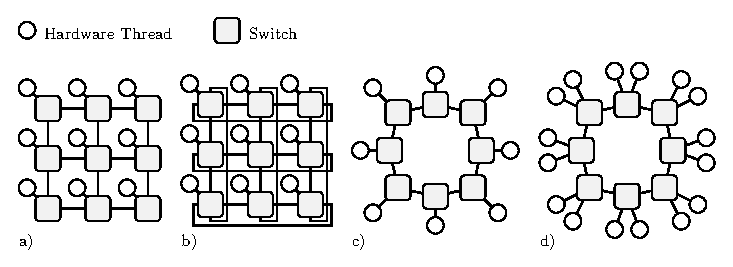
\includegraphics[width=\textwidth]{nocTopologies.eps}
  \caption{Examples of NoC topologies: a) Grid b) Torus c) Ring with one hardware thread per switch d) Ring with two hardware threads per switch}
  \label{nocTopologies.eps}
  \end{center}
\end{figure}

\subsection{\label{linkFlowMeasure}The Total Link Flow Measure}
In order to guarantee the required throughput for the hardware threads, each link in the NoC must be able to forward an individual worst-case data rate. We adapt the capacity of each link to its worst-case data rate by manipulating the number of parallel channels the link contains. We assume that the hardware resources needed by a link is approximately proportional to its number of parallel channels.

We define the \textit{total link flow} of a topology as the sum of the worst-case data rates on the individual links of the whole topology. According to the above argumentation, this measure is approximately proportional to the total hardware resources used by the links of the NoC. 

\paragraph{\label{linkFlowAlgorithm}Algorithm}
In order to estimate the resources used by the links of an NoC, we designed an algorithm that calculates the total link flow for an arbitrary NoC given the NoC's topology and routing policy. In this algorithm we assume, that each hardware thread is able to consume and produce data at exactly the rate 1.

The idea of the algorithm is to virtually send explorer packets from each hardware thread to all other hardware threads, containing the ID of the source and destination hardware thread. Every time a packet traverses a link, the link adds the source and destination ID pair to a link-local list. This list is then interpreted as a bipartide graph with the senders in one partition 	and the receivers in the other partition. The worst-case data rate of a link is then determined by the cardinality of the maximum matching of the bipartide graph.

Here is how the algorithm works:
\begin{enumerate}
\item Set up the network as a directed graph $G_{net}=(V,E)$ with
	\begin{enumerate}
		\item $V$ the set of all nodes $v$
		\item $E$ the set of all links $e=(v_i,v_j)$ able to forward packets from $v_i$ to $v_j$.
	\end{enumerate}
\item Let $E_{out,i}$ be the set of negative incident edges of node $v_i$.
\item For all nodes $v_i$ in $V$ select a routing policy $R_i:v_{dest}\rightarrow e_{out}$ where $v_{dest}\neq v_i$ is the destination of the routed packet and $e_{out} \in E_{out,i}$ is the outgoing link chosen to forward the packet.
\item Send explorer packets
	\begin{enumerate}
		\item All nodes $v_{src}\in V$ send exactly one packet $p=(v_{src},v_{dest})$ to all nodes $v_{dest}	\in V, v_{src}\ne v_{dest}$.
		\item All links $e_i \in E$ refer to a bipartide graph $G_{link,i}=(S_i\cup D_i,L_i)$. $S_i$, $D_i$ and $L_i$ are initialized as empty sets. Upon forwarding packet $p=(v_{src},v_{dest})$ on the link $e_i$, the link
		\begin{enumerate}
			\item adds $v_{src}$ to $S_i$ (if $v_{src}\not\in S_i$),
			\item adds $v_{dst}$ to $D_i$ (if $v_{dest}\not\in D_i$),
			\item adds the edge $(v_{src},v_{dest})$ to $L_i$.
		\end{enumerate}
	\end{enumerate}
	\item Select the worst case data rate on 	all links $e_i$
	\begin{enumerate}
		\item For the bipartide graph $G_{link, i}$ find a maximum matching $M_i$ (e.g. using the Hopcroft-Karp algorithm).
		\item From graph theory we know, that for a bipartide graph, the cardinality $|M_i|$ of a maximum matching is equal to the cardinality of the maximum flow $|f_i|$ from one partition of the graph to the other.
		\item The worst-case data rate on the link $e_i$ is therefore equal to $|M_i|$.
	\end{enumerate}
	\item The total link flow $f_{tot}$ of the given topology and routing policy is then $	f_{tot} = \sum_{v_i\in V} |M_i|$

\end{enumerate}


\paragraph{\label{linkFlowResults}Results}
We implemented the algorithm presented above using the Java programming language. Table~\ref{totalLinkFlowResults} presents the results for a set of topologies and routing algorithms. Additionally, figure \ref{totalLinkFlow.eps} shows a graphical visualization of the most representative values.

We see from these results, that the simplest version of the ring topology (with 1 functional block per switch) has a much higher total link flow than the grid topology. With an increasing number of functional blocks connected to the switches in the ring topology, the difference in the total link flow decreases more and more. Finally, the total link flow of the ring topology with 4 functional blocks per switch is comparable to the total link flow of the grid topology.

The most surprising result is that the total link flow of the grid topology is exactly the same as that of the torus topology. The total link flow of the various ring topologies is also independent of the chosen routing algorithm.

\begin{table}
\begin{center}
\begin{tabular}{|l|l|rrrrrrrr|}
\hline
	\multicolumn{2}{|l|}{Nodes} & 1 & 4 & 6 & 9 & 12 & 16 & 20  & 25 \\
\hline
\hline
	Topology & Routing & & & & & & & & \\
\hline
	Grid & XY & 0 & 8 & & 36 & & 96 & & 200 \\
	Torus & XY & 0 & 8 & & 36 & & 96 & & 200 \\
	Ring (1 FB/SW) & Unidirectional & 0 & 12 & 30 & 72 & 132 & 240 & 380 & 600\\
	Ring (1 FB/SW) & Bidirectional & 0 & 12 & 30 & 72 & 132 & 240 & 380 & 600\\
	Ring (2 FB/SW) & Unidirectional &0& 12 & 24 & 53 & 84 & 144 & 220 & 349\\
	Ring (3 FB/SW) & Unidirecitonal &0 & 10 & 18 & 36 & 60 & 110 & 159 & 248\\
	Ring (4 FB/SW) & Unidirectional &0 & 8 & 16 & 33 & 48 & 80 & 120 & 197\\
\hline
\end{tabular}
\caption{Total link flow of NoCs with a specific topology and routing algorithm.}
\label{totalLinkFlowResults}
\end{center}
\end{table}

\begin{figure}
  \begin{center}
		 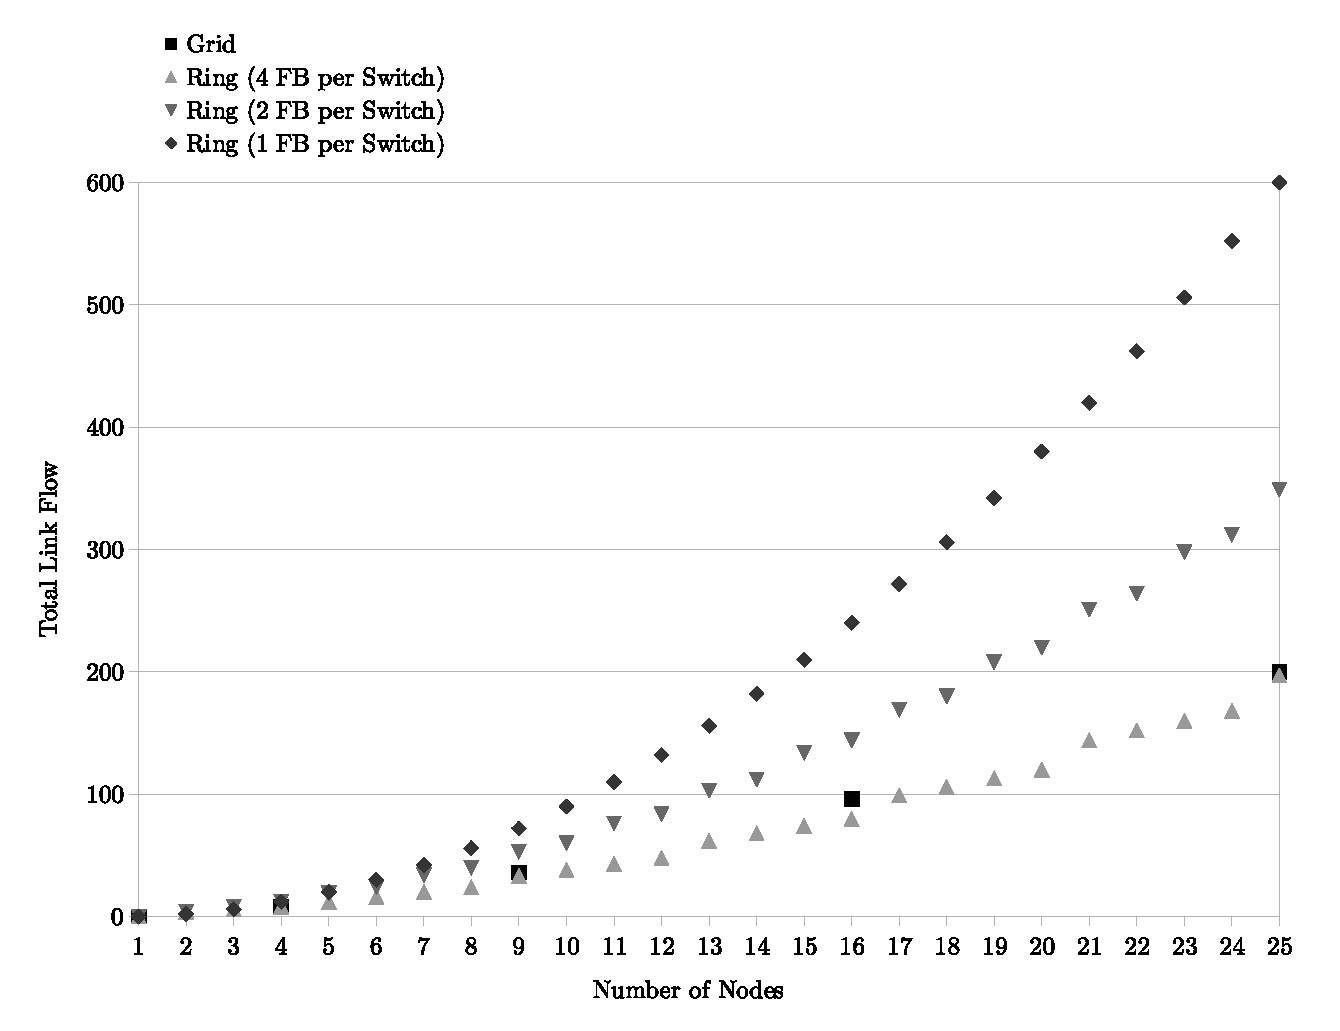
\includegraphics[width=\textwidth]{totalLinkFlow.eps}
  \caption{Total link flow of the ring and grid topology}
  \label{totalLinkFlow.eps}
  \end{center}
\end{figure}

\subsection{\label{evaluationOfTopologies:conclusion}Conclusion}
The evaluation of NoC topologies results in a trade-off decision. On one hand we have the grid topology with a relatively complex routing mechanism and a low resource consumption for the links. On the other hand we have the ring topology with a very simple routing mechanism and a high resource consumption for the links. The ring topology with multiple functional blocks per switch seems to be a good trade-off between these two extremes. We therefore decided to implement the ring topology with an adaptable number of functional blocks per switch. Figure~\ref{interconnectionInfrastructureRing.eps} shows an example of the resulting architecture with two functional blocks per switch and three parallel channels between the switches.
\begin{figure}
  \begin{center}
		 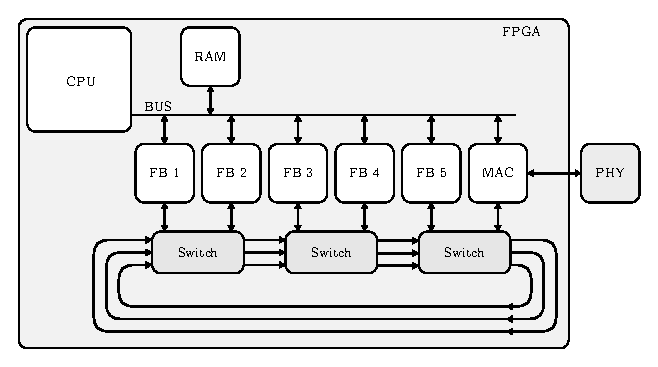
\includegraphics[width=\textwidth]{interconnectionInfrastructureRing.eps}
  \caption{An example of the resulting NoC topology: a ring with two functional blocks per switch and three parallel channels between the switches}
  \label{interconnectionInfrastructureRing.eps}
  \end{center}
\end{figure}


\section{\label{hwSwDataTransfer}Hardware - Software Data Transfer}
In sections~\ref{evaluationOfDesignPrinciples} and \ref{evaluationOfTopologies} we focused on the exchange of data between two hardware threads. In this section we now want to concentrate on the data transfer between hardware- and software threads. 

\subsection{Utilities provided by ReconOS}
\paragraph{Message Boxes} In ReconOS, a thread - either hardware or software - can write 32 bit words to a message box. These words stay in a message box until any thread reads them. The write and read access of message boxes is automatically thread-safe. When a thread reads from an empty message box, the corresponding system call blocks until another thread writes data into the message box. ReconOS raises an interrupt at the CPU whenever a data word is written to a message box. It is therefore not feasible to handle high volume data transfers with message boxes, since this would cause a very high interrupt load. Message boxes are more appropriate for notifying other threads about infrequent events.
\paragraph{Shared Memory}
ReconOS provides hardware and software threads with concurrent access to shared memory. Typically, a software thread allocates the shared memory segment and then sends the starting address of the segment to the hardware threads using message boxes. The access to shared memory is inherently not thread-safe. Therefore, threads must define appropriate critical sections when accessing the shared memory. The data transfer rate of shared memory is much higher than the data transfer rate of message boxes. However, threads waiting for new data are not notified about a write access of other threads and must therefore poll the shared memory.



\subsection{Distributed versus Centralized}
We can see from figure~\ref{interconnectionInfrastructureRing.eps} that the hardware threads are now at the same time connected to the NoC and the shared bus. The hardware threads can therefore simultaneously transfer packets to other hardware threads via the NoC and to software threads via the ReconOS interface.

% distributed
This distributed approach is not optimal in the case where two or more hardware threads send packets to the software at the same time. In this scenario, all sending hardware threads raise interrupts at the CPU for notifying the software thread about the availability of new data.

% centralized
In order to avoid this problem, we decided to implement a more centralized architecture. In this approach, two hardware threads form a \textit{hardware-to-software-} and a \textit{software-to-hardware gateway}, respectively. Hardware mapped functional blocks that want to transfer packets to a software thread send these packets via the NoC to the hardware-to-software gateway. The gateway is then responsible for transferring the packets to the software. The software-to-hardware gateway works just the same way. Software threads send packets to the software-to-hardware gateway which then redistributes the packets to their destination hardware thread using the NoC. Figure \ref{hwSwGateways.eps} visualizes this centralized architecture.

These gateways can aggregate multiple packets that have to cross the hardware/software boundary within a specific time interval and therefore reduce the total number of required interrupts. The higher latency of the packets caused by the additional transfer on the NoC is well compensated by the reduced interrupt handling time.

\begin{figure}
  \begin{center}
		 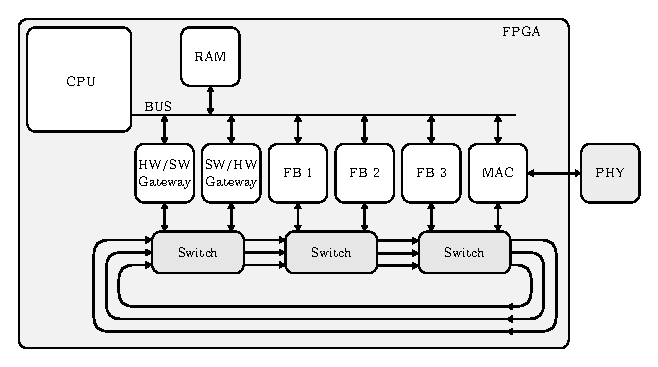
\includegraphics[width=\textwidth]{hwSwGateways.eps}
  \caption{Two dedicated hardware threads for a hardware-to-software and a software-to-hardware gateway, respectively}
  \label{hwSwGateways.eps}
  \end{center}
\end{figure}

\subsection{Ring Buffer}
The hardware-to-software gateway and the software-to-hardware gateway are very similar in concept. We therefore generalize the gateway's mechanism in order to reduce the documentation effort. Both gateways consist of a \textit{producer} thread and a \textit{consumer}. In the hardware-to-software gateway, the producer is a hardware thread and the consumer is a set of software threads. Conversely, in the software-to-hardware gateway, the producer is a set of software threads and the consumer is a hardware thread.

Both gateways transfer data across the hardware/software boundary by using ring buffers in the shared memory. The producer and the consumer both hold a copy of the read and write pointer of the ring buffer. When a packet is ready to be transferred, the producer first checks whether there is enough free space available in the ring buffer for the packet. If this is the case, the producer then writes the size of the packet and the actual packet to the shared memory. A padding block may be necessary to fill the gap between the end of the packet and the the next word offset. After this write procedure, the producer sets its write pointer to the first offset after the packet. Figure \ref{ringBufferPacketFormat.eps} illustrates the format of the packets in the ring buffer.

\begin{figure}
  \begin{center}
		 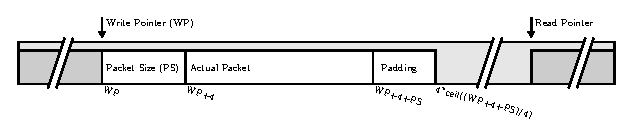
\includegraphics[width=\textwidth]{ringBufferPacketFormat3.eps}
  \caption{The format a packet in the ring buffer}
  \label{ringBufferPacketFormat.eps}
  \end{center}
\end{figure}
Eventually, the producer decides that it is reasonable to notify the consumer about the packets in the ring buffer. The producer then writes its current write pointer to a message box. Upon receiving a new write pointer via the message box, the consumer knows that the area between the read pointer and the newly received write pointer is filled with valid packets. After the consumer processed all packets in this area, it updates its read pointer with the value of the received write pointer. The consumer then writes its read pointer to another message box, which is read by the producer. When the producer receives the newly read pointer of the consumer, it knows that the corresponding area of the ring buffer can be used again for the transfer of new packets.

The tricky question is now: when should the producer initiate such an exchange of read and write pointers? The answer to this question is a trade-off. On one hand, we want to aggregate as much packets as possible in order to reduce the interrupt load. On the other hand, we need an upper bound for the latency of the packets. We further want to provide a non-blocking write access to the producer. We therefore require that a minimum amount of free space is always available in the ring buffer. Additionally, some packets may be very delay sensitive. We want to support these urgent packets and even allow them to decrease overall performance of the system. We therefore specify the following rules for the pointer exchange:
\begin{itemize}
\item The producer starts a timer when it writes a packet to the ring buffer for the first time after sending the write pointer to the consumer. An pointer exchange is initiated when this timer expires. This guarantees that the packets are not blocked in the ring buffer for more than one timer period.
\item After the producer has written a packet to the ring buffer, it checks the amount of free space in the ring buffer. If this value is below a specific threshold, the producer initiates a pointer exchange. This enables the producer to continue writing packets to the ring buffer during the pointer exchange procedure.
\item Delay sensitive packets have a specific flag set in their packet header. After writing such packets to the ring buffer, the producer immediately initiates a pointer exchange. 
\end{itemize}
















%** Results.tex: What were the results achieved including an evaluation
%
%\chapter{\label{results}Title}
The results from your evaluations.

%** Outlook.tex: What needs to be done further, what is planed
%
%\chapter{\label{outlook}Title}
What are the consequences of your work for future work?

%** Summary.tex: What have you achieved, what have you presented in this
%                document.  What are the highlights of your work.
%                It should conclude by a conclusion.
%\chapter{\label{summary}Title}
Sum up what you have done and recapitulate your key findings.



%** Switch to appendix-mode in Latex.
%
\appendix

%** I would like to have the appendices enumerated by Alphabetical
%   characters.
\renewcommand{\thepart}{\Alph{part}}

%** appendix.tex: Install instructions, configurations, test results,
%		simulation data, additional theoretical disquisitions, ...
%
%%%****************************************************************************
%** Copyright 2005 by Bernhard Tellenbach, <bernhard.tellenbach@airmail.ch>
%** Information is provided under the terms of the
%** GNU Free Documentation License <http://www.gnu.org/copyleft/fdl.html>
%****************************************************************************
%****************************************************************************
%** Last Modification: 2005-07-11 1600
%** 2005-07-11	Updated the syntax to match the current nomencl packet
%****************************************************************************

\chapter{\label{appendixA}Title}


\section{\label{chapterA:section1}Section 1}

\begin{verbatim}
All is presented exactely the way you write it.

Page boundaries are not checked.....................................................................................

\end{verbatim}

\chapter{\label{appendixB}Title}


%Entries for the list of abbrevations:
%
%To generate the list of abbrevations, execute:
%makeindex Thesis.nlo -s nomencl.ist -o Thesis.nls
%
%If you are using TeXniCenter, specify:
%"%bm.nlo" -s nomencl.ist -o "%bm.nls"
%as beeing the argument list for makeindex.
%---------------------------------------------------------------------------------------------------------
%For old nomencl package uncomment this:
%\printglossary
%For new nomencl package uncomment this:
\printnomenclature

\abbrev{XCA}{\markup{X}tremely \markup{C}ool \markup{A}bbrevations}




%** Timetable.tex: Timetable you worked out.
%
%\chapter{\label{timetable}Title}
Here may come your thesis schedule (the original plan and ev. the actual outcome).

%** Originalproblem.tex: The problem statement you received.
%
\chapter{\label{originalproblem}Original Task Description}
%
\includegraphics[width=\linewidth]{TIKETHhdr.pdf}
	
%	\begin{center}
%	\LARGE ~\\
%	\LARGE Master Thesis\\
%	\large ~\\
%	\huge A Dynamic Hardware Architecture\\for Future Networks
%        \large ~\\
%        \large ~\\
%	\LARGE Richard Huber\\
%	\large ~\\
%	\large Advisor: 	Ariane Keller, ariane.keller@tik.ee.ethz.ch\\
%	\large Co-Advisor:	Dr. Stephan Neuhaus, stephan.neuhaus@tik.ee.ethz.ch \\
%	\large Co-Advisor:	Daniel Borkmann, daniel.borkmann@tik.ee.ethz.ch \\
%	\large Professor: Prof. Dr. Bernhard Plattner, plattner@tik.ee.ethz.ch \\
%	\large ~\\
%	\large December 2011 - June 2012
%	\vspace{10mm}
%	\end{center}

\section{Introduction}
This master thesis is in the context of the EPiCS project.
The goal of the EPiCS project is to lay the foundation for engineering the novel class of proprioceptive computing systems.
Proprioceptive computing systems collect and maintain information about their state and progress, which enables self-awareness by reasoning about their behaviour, and self- expression by effectively and autonomously adapting their behaviour to changing conditions. Concepts of self-awareness and self-expression are new to the domains of computing and networking; the successful transfer and development of these concepts will help create future heterogeneous and distributed systems capable of efficiently responding to a multitude of requirements with respect to functionality and flexibility, performance, resource usage and costs, reliability and safety, and security. 

In this thesis we focus on the networking aspect of EPiCS which we call \textit{EmbedNet}. EPiCS uses the network architecture developed in the ANA project as a basis. 
The ANA network architecture is a novel architecture that enables flexible, dynamic, and fully autonomous formation of network nodes.
In the EPiCS project we develop the ANA architecture further. On the one hand we will develop mechanisms to adapt the functionality provided by the protocol stack at runtime, on the other hand we will develop mechanisms that map the networking functionality dynamically to either hardware or software.

The objective of this Masters Thesis is to refine the hardware architecture and the hardware/software interface of EmbedNet. 


\section{Assignment}
This assignment aims to outline the work to be conducted during this thesis. 
The assignment may need to be adapted over the course of the project. 

\subsection{Objectives}
The goal of this Master thesis is to develop a hardware architecture for future dynamic protocol graphs. 
The developed architecture has to partition networking functionality into individual blocks. 
The architecture should allow for the dynamic reconfiguration of whole networking blocks as well as for the runtime configuration of communication parameters in the networking blocks.
An interconnect between the functional blocks should be provided that allows for the forwarding of packets at line rate. The transmit data path should not interfere with the reception data path.

\subsection{Tasks}
This section gives a brief overview of the tasks the student is expected to perform towards achieving the objective outlined above. 
The binding project plan will be derived over the course of the first three weeks depending on the knowledge and skills the student brings into the project.

\subsubsection{Familiarization}
\begin{itemize}
	\item Study the available literature on ANA, EmbedNet and Reconos [1, 2, 3, 4].
	\item Setup a FPGA development environment with the Xilinx tools 12.3 (exact) and ModelSim SE version 6.1f (or higher).
        \item Familiarize yourself with git/github and clone the reconos source code repository [5].
        \item Install the eCos source code and cross compile toolchain [6].
        \item Verify your toolchain by running first the sort\_demo\_thermal and then the pr\_demo.
	\item In collaboration with the advisor, derive a project plan for your master thesis. 
		Allow time for the design, implementation, evaluation, and documentation of your software.
\end{itemize}

\subsubsection{Architecture and hardware design}
\begin{itemize}
        \item Develop a dedicated communication interface between the different hardware networking blocks. Adapt the hardware blocks where needed. 
        The interface should be able to forward data at line rate (1Gbit/s). Transmission and reception direction should be treated independently. 
        The interface should support different priorities of either sending networking blocks or individual packets. 
        \item Develop a configuration interface for the hardware networking blocks. 
        Each hardware block needs to be configured with the information required for forwarding the individual packets to the next protocol. 
        The configuration interface should be able to set, delete, and replace configuration entries. The configuration should be initiated by a software program. 
        \item Develop a data path for sending data between hardware and software networking blocks. 
        Consider using two ring buffers per networking block, one for packets to be transmitted and one for packets to be received. 
        The reader/writer synchronization should be handled properly. An interface should be developed to send and receive packets from software.
        \item Optional: Adapt the data path to work with the LANA protocol stack [7].
        \item Optional: Develop a monitoring framework for the measurement of hardware parameter such as temperature, utilisation or power consumption. 
        The framework should collect the data in hardware and make them accessible to a software program.  
\end{itemize}

\subsubsection{Implementation}
\begin{itemize}
        \item Determine an appropriate version control system. The EPiCS project is hosted at github. You might want to put your code in the same repository.
	\item Implement a static version of the dedicated communication interface together with some dummy networking blocks for validation purposes.
        \item Add the possibility for partial reconfiguration of hardware networking blocks to the communication interface.
        \item Implement the configuration interface. 
        Depending on the overall EPiCS project status use either the eCos operating system or the Linux operating system (preferred).
        \item Implement the data path for the hw/sw interface.
        Depending on the overall EPiCS project status use either the eCos operating system or the Linux operating system (preferred).
        \item Optional: Implement the interface to LANA.
        \item Optional: Implement the monitoring framework.
\end{itemize}

\subsubsection{Validation}
\begin{itemize}
	\item Validate the correct operation of your implementation after each implementation step. 
        Use for your evaluation different packet sizes (short, long, even or odd number of bytes, etc.).
	\item Check the resilience of the implementation, including its configuration interface, to uneducated users.
\end{itemize}

\subsubsection{Evaluation}
\begin{itemize}
	\item Do a performance evaluation of your implementation.
        \item Optional: Determine the bottlenecks of your implementation.
        \item Optional: Do a performance comparison between packet forwarding for different combinations of hardware and software networking functional blocks.
\end{itemize}

\subsubsection{Documentation}
\begin{itemize}
	\item Appropriate source code documentation.
        \item Write a step-by-step how to that describes the compilation of your code, the loading of the code into the hardware and the execution of your code.
	\item Write a documentation about the design, implementation, validation and evaluation of your work.
\end{itemize}


\section{Milestones}
\begin{itemize}
    \item Provide a "project plan" which identifies the mile stones. 
    \item Two intermediate presentations: Give a presentation of 10 minutes to the professor and the advisors. 
    			In this presentation, the student presents major aspects of the ongoing work including results, obstacles, and remaining work.
    \item Final presentation of 15 minutes in the CSG group meeting, or, alternatively, via teleconference. 
    			The presentation should carefully introduce the setting and fundamental assumptions of the project. 
    			The main part should focus on the major results and conclusions from the work.
    \item Any software that is produced in the context of this thesis and its documentation needs to be delivered before conclusion of the thesis. 
    	This includes all source code and documentation.
    	The source files for the final report and all data, scripts and tools developed to generate the figures of the report must be included. 
    	Preferred format for delivery is a CD-R.
    \item Final report. The final report must contain a summary, the assignment, the time schedule and the Declaration of Originality. Its structure should include the following sections: Introduction, Background/Related Work, Design/Methodology, Validation/Evaluation, Conclusion, and Future work. Related work must be referenced appropriately.
\end{itemize}

\section{Organization}
\begin{itemize}
	\item 	Student and advisor hold a weekly meeting to discuss progress of work and next steps. 
		The student should not hesitate to contact the advisor at any time. 
		The common goal of the advisor and the student is to maximize the outcome of the project.
	\item 	The student is encouraged to write all reports in English; German is accepted as well. 
    	\item	The core source code will be published under the GNU general public license.
\end{itemize}

\section{References}
[1] ReconOS: Multithreaded Programming for Reconfigurable Computers: Description of the hardware/software architecture
\newline
[2] Reconifgurable Nodes for Future Networks: Description of how we would like to use the hw/sw architecture to build reconfigurable networks
\newline
[3] The Autonomic Network Architecture (ANA): Description of the ideas and sw prototype for configurable networks
\newline
[4] https://github.com/EPiCS/epics-org/blob/master/deliverables/D3-1\_Architecture\_And\_Tool\_Flow/D3-1\_Architecture\_And\_Tool\_Flow.pdf
\newline
[5] https://github.com/EPiCS/reconos/
\newline
[6] webpage: ecos.sourceware.org, a version that is compliant with reconos is in the github repository, cross compilation tools: gcc-4.1.2 glibc-2.3.6
\newline
Webpages:
\newline
http://www.ana-project.org
\newline
http://www.epics-project.eu
\newline
http://www.reconos.de



\bibliography{bibliography}{}
\bibliographystyle{plain}

%** end the document environment
\end{document}
